%


\begin{appendices}

%Some Table of Contents entry formatting
\addtocontents{toc}{\protect\renewcommand{\protect\cftchappresnum}{\appendixname\space}}
\addtocontents{toc}{\protect\renewcommand{\protect\cftchapnumwidth}{6em}}

%Begin individual appendices, separated as chapters

\chapter{Thermodynamic costs of dynamic function in active soft matter}




\section{Introduction}

Living matter performs a remarkable variety of complex functions (Fig.~\ref{fig:1}a): chloroplasts within plants capture energy from sunlight and convert it into chemical fuels and structural materials; muscle tissue powers organisms to move and to transport matter throughout their interiors; the cytoskeleton incessantly reconfigures its structural components, enabling cells to adapt their mechanical properties to their environment; the skin of vertebrate organisms provides a protective barrier that repairs itself when damaged and maintains its function despite wear; nervous tissue uses complex signaling networks to sense environmental inputs and compute intelligent outputs.  Perhaps most remarkably, all organisms grow and replicate these living materials to escape the unrelenting pull toward thermodynamic equilibrium (i.e., death). These functions---and the many others not listed---would be highly desirable to achieve in synthetic material systems, and yet we remain far from this goal. Why?

%%%%%%%%%%%%%%%%%%%%%%%%%%
\begin{figure}[!p]
     \centering
     \includegraphics[width= 8.5 cm]{figures/A5_Figure1.pdf}
     \caption{(a) Examples of dynamic functions in living matter. Left to right, top to bottom: chloroplasts, skeletal muscle, cell cytoskeleton, rhinoceros skin, neuronal network, bacterial colony. (b) Dynamic functions require the coupling of complex structures and dissipative processes---here, a kinesin motor protein bound to a microtubule does work powered by ATP hydrolysis. All images are public domain. }
%Figure source left to right , up to bottom
%https://en.wikipedia.org/wiki/Chlorophyll
%https://en.wikipedia.org/wiki/Muscle
%https://www.cshlpress.com/default.tpl?cart=1537454398711019648&fromlink=T&linkaction=full&linksortby=oop_title&--eqSKUdatarq=1107
%https://en.wikipedia.org/wiki/Rhinoceros
%https://www.flickr.com/photos/gehealthcare/4253587827/
     \label{fig:1}
 \end{figure}
%%%%%%%%%%%%%%%%%%%%%%%%%%

Materials science has traditionally focused on controlling structure and composition as the primary route to achieving function in materials. In this paradigm, material function (e.g., mechanical strength or electrical conductivity) is determined by the spatial organization of material components (e.g., atoms, molecules, nanoparticles, etc.). This approach has been widely successful. We can now create materials with heterogeneous structure and composition on length scales spanning molecular to macroscopic dimensions (e.g., an integrated circuit).  These structures form the material basis for the modern world. However, control over structure alone is insufficient to realize the \emph{dynamic functions} characteristic of living matter.

In addition to structural complexity, living matter is further distinguished by the presence of dissipative \emph{processes} that organize and animate material components in space and time to achieve dynamic function. For example, the complex structure of a kinesin motor protein is unrivaled by that of synthetic macromolecules; however, its ability to perform mechanical work requires energy input and temporal control provided by chemical reactions (Fig.~\ref{fig:1}b). More generally, the dynamic functions of living matter require integration of structures \emph{and} processes to drive material organization in space and time.  Such organization is not possible at thermodynamic equilibrium but instead requires flows of energy and matter to create and maintain spatiotemporal order among the system's components.  These currents dissipate energy as heat and waste, thereby increasing the entropy of the surroundings.  In short, dynamic functions have a thermodynamic cost: living matter needs to eat. 

The creation of synthetic material systems that perform dynamic functions requires a different paradigm---one in which material structures are coupled to and animated by networks of dissipative processes.  Progress towards this challenging goal is underway in a variety of fields.  In statistical physics, interest in non-equilibrium thermodynamics \cite{de2013non} has been renewed by the discovery of non-equilibrium principles---such as fluctuation theorems \cite{jarzynski2011equalities} and uncertainty relations \cite{Seifert2018}---that describe the behavior of small (fluctuating) systems driven away from equilibrium \cite{Seifert2012,Marsland2018}.  These principles are being applied to elucidate the biophysical mechanisms of cellular oscillators \cite{Cao2015,Barato2016}, molecular motors \cite{Pietzonka2016,Hess2017}, dissipative assemblies \cite{Nguyen2015, marsland2018active}, and sensory adaptation \cite{Lan2012,Tu2018} among others.  The study of active matter \cite{Marchetti2013} shifts the focus from individual driven components such as molecular motors to their large scale collective behaviors \cite{Needleman2017, Doostmohammadi2018}. The creation of self-propelled particles---so-called active colloids \cite{Bechinger2016, illien2017fuelled, Zhang2017}---provides synthetic realizations of active matter with emerging opportunities as autonomous microrobots \cite{Palagi2018, han2018engineering}. The chemical synthesis of molecular motors \cite{kassem2017artificial,Astumian2017} and dissipative assemblies \cite{VanRossum2017,De2018} highlight the potential for systems chemistry \cite{Ashkenasy2017}, in which molecular systems are guided by dissipative networks of chemical reactions \cite{Epstein2016, Grzybowski2017}. Inspired by living matter, these diverse pursuits promise advances in molecular systems \cite{merindol2017materials}, nanotechnology \cite{Grzybowski2016},  biomaterials \cite{tibbitt2017living}, and even artificial cells \cite{Yewdall2018}.

Here, we integrate elements from these different fields to provide an idiosyncratic perspective on the creation of \emph{active soft matter}. This label refers to systems of molecules, polymers, and particles in liquid environments that move and interact with characteristic energies comparable to the thermal energy at room temperature. Moreover, these materials are driven and maintained away from equilibrium by external thermodynamic forces, resulting in flows of matter and energy needed to perform dynamic functions. This broad definition, encompassing much of cell biology, active matter, and systems chemistry, is united by a common framework---that of, \emph{stochastic thermodynamics} \cite{Seifert2012}---which describes small driven systems immersed in a heat bath.  The dynamics of such systems are described by stochastic processes, in which the concepts of work, heat, and entropy production are described at the level of fluctuating trajectories. Even far from equilibrium, these fluctuating quantities obey universal relations, which establish fundamental trade-offs between the rate of energy dissipation and performance metrics such as precision, efficiency, and speed. 

In pursuit of active soft matter, we advocate a constructionist perspective summarized by Richard Feynman: ``What I cannot create, I do not understand.'' If we seek to understand the inner workings of living matter, we should strive to create synthetic analogs---perhaps greatly simplified---that perform similar dynamic functions. These analogs or ``models'' can be material or conceptual---for example, a synthetic molecular motor or a mathematical description thereof.  In both cases, the construction of the model, marked by false starts and dead ends, teaches us what is necessary and what is superfluous to achieving the targeted function.  Moreover, by building systems that push the limits of performance, we discover universal bounds that constrain the operation of biological and non-biological matter alike.

The constructionist approach should be directed and motivated by the pursuit of dynamic function to avoid the creation of models for their own sake without generating broader insights.  Living matter dissipates energy to perform remarkable functions; however, dissipation alone is unremarkable. The Reader would not be impressed by a ``life-like'' paper weight that requires a steady supply chemical fuel for its operation. Many functions---like keeping documents in order---can and should be achieved without dissipating energy. Instead of focusing on dissipation as a hallmark of living matter, we should shift our attention to the dynamic functions we aim to achieve.  How can we make a chemical clock that oscillates more reliably?  How can we convert chemical energy to mechanical work more efficiently?  How can we assemble and disassemble material structures more quickly?  The pursuit of these and other dynamic functions in active soft matter can serve to orient and guide our exploration of this exciting new field.

In this spirit, the present Review is organized around four dynamic functions under the headings of (1) keeping time, (2) powering motion, (3) building structures, and (4) making copies. For each function, we present a simple kinetic model that identifies the essential ingredients and illustrates the fundamental trade-offs between dissipation and performance. These examples are often adapted from biophysical models and repackaged in the context of synthetic materials such as colloidal machines, nanoparticle assemblies, and DNA nanotechnology. In this way, the complex functions of biology are simplified into minimal models, which in turn guide the design of bioinspired, synthetic materials. Building on general lessons from the models, we discuss recent progress and challenges in creating active soft matter capable of dynamic functions. Our coverage of the recent literature is far from comprehensive. Instead, we aim to bridge experimental efforts in active soft matter and theoretical advances from stochastic thermodynamics to inform future research on material systems inspired by living matter. To this end, we begin with a brief introduction to the stochastic thermodynamics of non-equilibrium steady-states and the thermodynamic uncertainty relation  \cite{Barato2015, Gingrich2016, Pietzonka2016b}. It is our hope that this cross-disciplinary perspective will spark new connections among communities interested in understanding, designing, and constructing dissipative material systems.

%%%%%%%%%%%%%%%%%%%%%%%%%%
%%%%%%%%%%%%%%%%%%%%%%%%%%
\section{Stochastic Thermodynamics}

The kinetic models presented below are described by the framework of stochastic thermodynamics, which considers the fluctuations of thermodynamic quantities in small systems driven out of equilibrium by external forces \cite{Seifert2012, VanDenBroeck2015, Ciliberto2017} (see \cite{Seifert2018} for a recent and accessible introduction to the field).  Here, we briefly summarize the concepts relevant to our discussion of dynamic function. We consider systems at constant temperature maintained in non-equilibrium steady-states by chemical reactions or other thermodynamic forces.  Our choice to exclude phenomena involving time-varying fields \cite{Barato2016,Barato2017b} or thermal gradients \cite{Pietzonka2018} is one of convenience and should not be viewed as a limitation of stochastic thermodynamics.  Systems at steady-state obey a universal non-equilibrium principle known as the thermodynamic uncertainty relation \cite{Barato2015, Gingrich2016, Pietzonka2016b}, which bounds the magnitude of current fluctuations by the rate of entropy production.  This recent advance in non-equilibrium statistical mechanics has important implications for the performance of small machines and therefore the design of active soft matter.

%%%%%%%%%%%%%%%%%%%%%%%%%%
\subsection{Markovian Networks}

We consider a coarse-grained description of the system in which the many microstates are partitioned into $N$ mesostates, each characterized by an equilibrium free energy $F_i$ for $i=1\dots N$.  The validity of this description relies on the separation of time scales for transitions within each mesostate (fast) and between different mesostates (slow).  At equilibrium, the probability of finding the system in the $i^{\text{th}}$ mesostate (henceforth ``state'') is given by the Boltzmann distribution, $p_i \propto \exp(-F_i)$. For notational convenience, we have set Boltzmann constant $k_B$ and the temperature $T$ to unity, such that all energies are given in units of the thermal energy $k_B T$.  At equilibrium, there are no net currents between any two states: the current $k_{ij} p_i$ from state $i$ to $j$ is equal to the current $k_{ji} p_j$ from state $j$ to $i$.  This condition of detailed balance implies that the transition rates $k_{ij}$ and $k_{ji}$ are related  at equilibrium as $\ln(k_{ij}/k_{ij})=F_i-F_j$. 

In driven systems, the application of thermodynamic forces---also called affinities---result in steady currents through the network of states.  A network of $N$ states connected by $E$ edges with non-zero transition rates ($k_{ij}\neq 0$) has $E-N+1$ independent currents, one for each fundamental cycle of the network \cite{schnakenberg1976network}.  The fluctuating current $X_{\beta}(t)$ around the cycle $\beta$ counts the number of cycle completions, increasing or decreasing by 1 on completion of the forward or reverse cycle, respectively.  In addition to the integrated current $X_{\beta}(t)$, the average current $J_{\beta}$ measures the number of cycle completions per unit time,
\begin{equation}
    J_{\beta} \equiv \langle X_{\beta}(t)\rangle / t
\end{equation}
where the brackets indicate an average over stochastic trajectories at steady-state.  Alternatively, the average current can be computed from the steady-state occupancy probabilities $p_i$ as $J_{\beta} = k_{ij} p_i - k_{ji} p_j$, where the edge $ij$ corresponds to a particular transition used in defining the set of fundamental cycles (see \cite{schnakenberg1976network} for details).  As at equilibrium, the occupancy probabilities at steady-state are defined by the set of linear equations, $k_{ij} p_i = k_{ji} p_j$.

The thermodynamic affinity $\mathcal{A}_{\beta}$ driving the cycle currents describes the decrease in free energy of the surroundings upon completion of the cycle $\beta$.  For example, the affinity of a cycle that consumes one ATP molecule and produces one ADP molecule is equal to the difference in chemical potentials of ATP and ADP in the surrounding reservoirs, $\mathcal{A}_{\beta}=\mu_{\text{ATP}}-\mu_{\text{ADP}}$.  In general, a single cycle may be associated with multiple processes (e.g., chemical reactions, mechanical motions) that contribute to its overall affinity $\mathcal{A}_{\beta}$.  To account for this possibility, we introduce a generalized distance $d^{\beta}_{ij}$ that describes the fraction of the cycle affinity $\mathcal{A}_{\beta}$ associated with the particular transition $i\rightarrow j$.  Considering both the system and its surroundings, the condition of detailed balance implies the following relation between the forward and reverse transition rates
\begin{equation}
    \ln\left(\frac{k_{ij}}{k_{ji}}\right) = \sum_{\beta} d^{\beta}_{ij} \mathcal{A}_{\beta} + F_i - F_j 
\end{equation}
During the transition $i\rightarrow j$, the fluctuating current $X_{\beta}(t)$ increases by the generalized distance $d^{\beta}_{ij}$; the fluctuating entropy change in the surrounding medium $s_m(t)$ increases by the increment $d^s_{ij} = \ln(k_{ij}/k_{ji})$.  The average rate of entropy production $\sigma$ is defined as 
\begin{equation}
    \sigma \equiv\langle s_m(t)\rangle / t = \sum_{\beta}\mathcal{A}_{\beta} J_{\beta} \label{eq:entropy}
\end{equation}
which is positive for non-equilibrium steady-states and zero at equilibrium.  For the isothermal systems considered here, the rate of entropy production is equivalent to the rate of energy dissipation.  We use these terms interchangeably in our discussion of the thermodynamic cost of dynamic functions.  

%%%%%%%%%%%%%%%%%%%%%%%%%%
\subsection{Thermodynamic Uncertainty Relation}

At the non-equilibrium steady-state, general results regarding the magnitude of fluctuations can be derived using techniques from large-deviation theory \cite{Touchette2009}. In particular, the thermodynamic uncertainty relation \cite{Barato2015,Gingrich2016} provides a universal bound on rate of dissipation required to achieve a desired level of precision in the fluctuating current $X_{\beta}(t)$. The precision is characterized by the scaled variance of the current $X_{\beta}(t)$, which provides a measure of uncertainty for the cyclic process,
\begin{equation}
    \epsilon^2_{\beta} \equiv \frac{\langle X_{\beta}^2 \rangle -\langle X_{\beta} \rangle^2 }{\langle X_{\beta} \rangle^2} = \frac{2 D_{\beta}}{J^2_{\beta} t}
\end{equation}
Here, $D_{\beta}\equiv ( \langle X_{\beta}^2 \rangle -\langle X_{\beta} \rangle^2) / t$ is the dispersion of the process, which approaches a constant value in the limit of long times.  Additionally, the cost of running this process for a time $t$ is equal to the average amount of entropy produced (or energy dissipated), $\mathcal{C} = \sigma t$. The thermodynamic uncertainty relation describes the fundamental trade-off between precision and dissipation for any Markov process
\begin{equation}
     \mathcal{C}\epsilon^2_{\beta} = \frac{2\sigma D_{\beta}}{J_{\beta}^2} \geq 2 \label{eq:TUR}
\end{equation}
Achieving greater precision (smaller $\epsilon_{\beta}^2$) comes only at the expense of higher cost (larger $\mathcal{C}$).  

The uncertainty relation (\ref{eq:TUR}) is saturated near equilibrium, at which the affinities $\mathcal{A}_{\beta}$ vanish. For large affinities characterizing ``far-from-equilibrium'' processes, there exist stronger but less general bounds for networks of certain simple topologies \cite{Pietzonka2016b}.  In particular, for a single cycle with $N$ states, the uncertainty relation is bounded by the affinity-dependent inequality  
\begin{equation}
    \mathcal{C}\epsilon^2 \geq \frac{\mathcal{A}}{N}\coth\left(\frac{\mathcal{A}}{2N}\right) \geq 2 \label{eq:unicycle}
\end{equation}
As illustrated in the example below, such bounds may be tighter or looser depending on the specific transition rates characterizing the system dynamics. 

%%%%%%%%%%%%%%%%%%%%%%%%%%
\subsection{Tutorial example: An electromechanical oscillator}

To demonstrate the mechanics of building and interrogating a simple kinetic model, we consider the dynamics of an electromechanical oscillator that shuttles charge between two electrodes subject to an applied voltage $V$ (Fig.~\ref{fig:KeepingTime}a). This system has been studied previously at the microscale as an electric motor for powering unit operations in microfluidic systems \cite{bishop2018contact,drews2015contact}.  Here, we describe an analogous system at the nanoscale, in which a particle (or molecule) transitions repeatedly between two charged states, $+e$ and $-e$, where $e$ is the elementary charge.  These transitions are assumed to occur only when the particle is located near the surface of either electrode.  The system is therefore modeled by $N=4$ discrete states corresponding to the two particle locations and two particle charges (Fig.~\ref{fig:KeepingTime}a).  For simplicity, we assume that the system is symmetric such that the free energy of the positively charged particle at the negatively biased electrode (state 1) is the same as that of the negatively charged particle at the positively biased electrode (state 3).  These states (1 and 3) are lower in energy than the others (2 and 4) by a common factor $\Delta F>0$, which implies that the charged particle moves spontaneously towards the oppositely biased electrode (Fig.~\ref{fig:KeepingTime}b).

%%%%%%%%%%%%%%%%%%%%%%%%%%
\begin{figure}[p!]
    \centering
    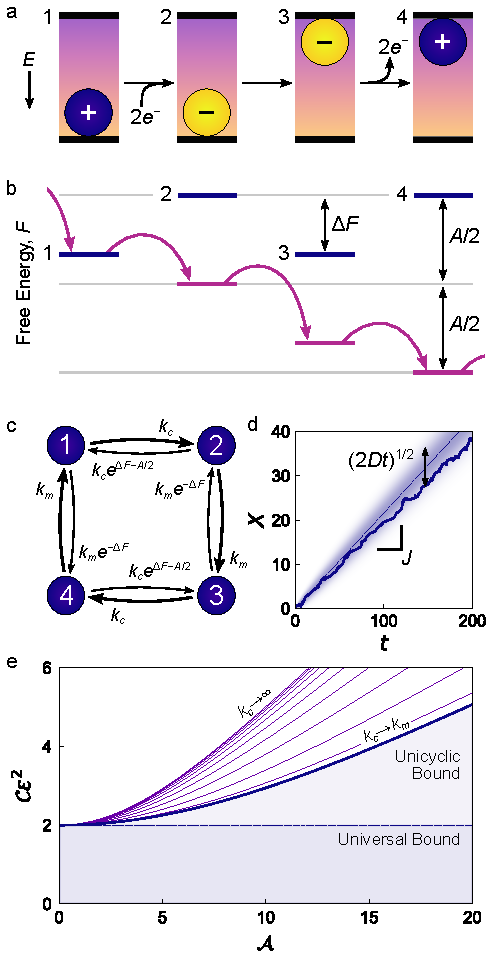
\includegraphics{figures/A5_KeepingTime.pdf}
    \caption{\textbf{Keeping Time.}(a) A 4-state Markov model of an electromechanical oscillator moving between two electrodes. (b) Free energy diagram showing the energies of the four states (blue) and the total energy of the system and its surroundings (purple). The arrows show how the total energy decreases by $\mathcal{A}$ during one cycle. (c) Markov network showing the relevant transition rates. (d) Fluctuating current $X(t)$ as a function of time for $\mathcal{A}=8$, $\Delta F=2$, and $k_c= 1$.  The shaded region shows the distribution for $X(t)$ as characterized by the average rate $J$ and dispersion $D$. (e) Computed product of the cost $\mathcal{C}$ and uncertainty $\varepsilon^2$ as a function of the affinity $\mathcal{A}$ for different values of the charging rate $k_c$ (purple curves).  The product $\mathcal{C}\epsilon$ is greater than the universal bound (\ref{eq:TUR}) and the unicyclic bound (\ref{eq:unicycle}). }
    \label{fig:KeepingTime}
\end{figure}
%%%%%%%%%%%%%%%%%%%%%%%%%%

The network is characterized by a single cycle with affinity $\mathcal{A}= 2 e V / k_B T$, corresponding to the transfer of 2 elementary charges down the potential difference $V$. The generalized distances described above are given by $d_{12}=d_{34}=1/2$ and $d_{32}=d_{41}=0$.  Transitions with $d_{ij}\neq0$ are coupled to the external reservoirs (electrodes) via charge transfer processes that allow for driving the system to higher energy states (Fig.~\ref{fig:KeepingTime}b).  Note, however, that the total energy of the system \emph{and} its environment decreases by an amount $\mathcal{A}$ during each cycle.  At steady-state, this thermodynamic force drives an average current $J$ which increases (nonlinearly) with the affinity $\mathcal{A}$.    

In addition to the network topology and energetics, the system's dynamics are determined by kinetic rate constants that reflect the speed of the different transitions. Accounting for the conditions of detailed balance and symmetry, the present model requires two such rate constants: one for charge transfer $k_c$ and another for particle motion $k_m$ (Fig.~\ref{fig:KeepingTime}c). We choose to measure time in units of $k_m^{-1}$ and thus set the rate constant $k_m$ to unity. The dynamics of the model is specified by three (dimensionless) parameters: the driving affinity $\mathcal{A}$, the free energy difference $\Delta F$, and the remaining rate constant $k_c$.  Figure \ref{fig:KeepingTime}d shows one realization of the fluctuating current $X(t)$ for $\mathcal{A}=8$, $\Delta F=2$, and $k_c= 1$.  The current increases at an average rate $J$ with dispersion $D$, which are computed analytically following the method of Koza \cite{koza1999general} (see also \cite{Pietzonka2016b}).

%%%%%%%%%%%%%%%%%%%%%%%%%%
%%%%%%%%%%%%%%%%%%%%%%%%%%
\section{Dynamic Functions}

Armed with the framework of stochastic thermodynamics, we now consider the theoretical analysis and synthetic realization of four dynamic functions in active soft matter: (1) keeping time, (2) powering motion, (3) building structures, and (4) making copies.

%%%%%%%%%%%%%%%%%%%%%%%%%%
\subsection{Keeping Time}

Biochemical oscillations are critical in controlling the timing of dynamic functions within living matter.  In particular, the different circadian rhythms allow organisms to anticipate and prepare for periodic changes in their environment such as light-dark cycles. The ability to keep accurate time enables organisms to more effectively harness environmental resources (e.g., light and food) and coordinate internal processes \cite{Sharma2003}. The benefits of ``keeping time'' come only at a thermodynamic cost \cite{Cao2015, Barato2016} in the form of energy dissipation. The thermodynamic uncertainty relation (\ref{eq:TUR}) establishes the universal trade-offs between the precision of small clocks and the energy currents required for their operation \cite{Barato2016}.  Here, we discuss these trade-offs in the context of a model Brownian clock---namely, the electromechanical oscillator introduced in the previous section.  We identify strategies for achieving optimal performance and highlight some recent progress in the design of synthetic oscillators. 

%%%%%%%%%%%%%%%%%%%%%%%%%%
\subsubsection{A Brownian Clock}

The electromechanical oscillator introduced in Figure \ref{fig:KeepingTime} provides a simple example of a Brownian clock \cite{Barato2016} where each cycle measures one ``tick'' of mean duration $J^{-1}$.  In using this clock to measure a specified time interval $\mathcal{T}$, we consider two performance metrics: the temporal precision $\epsilon^2$ and the thermodynamic cost $\mathcal{C}$.  First, an effective clock must be sufficiently precise.  For example, the timing of Olympic sprinters requires precision better than $\epsilon=10^{-3}$ to measure a 10 s interval accurate to 0.01 s.  Without this precision, the clock is useless: all sprinters finish the race in $10\pm1$ s.  The thermodynamic uncertainty relation states that temporal precision can be achieved only at a thermodynamic cost.  Here, the cost of running the clock is equal to the average amount of energy supplied to the electromechanical oscillator, $\mathcal{C}= J\mathcal{A}\mathcal{T}$.  The minimum cost of any Brownian clock is $\mathcal{C}_{\min} = 2/\epsilon^2$.  Timing the hundred meter dash requires a minimum energy input of more than $10^{6}$ times the thermal energy.

Real clocks may operate at costs substantially higher than this theoretical minimum.  Kinetic models are therefore useful in guiding improvements in system performance. One approach is reducing the driving affinity $\mathcal{A}\rightarrow 0$ to operate close to thermodynamic equilibrium (Fig.~\ref{fig:KeepingTime}e).  While thermodynamically efficient, this regime is often impractical as the speed of the clock slows to zero, $J(\mathcal{A})\rightarrow0$.  As a result, long times are required to achieve the desired precision---specifically, $\mathcal{T}=2D/J^2\epsilon^2\rightarrow\infty$ for constant $D$ and $\epsilon^2$.  In the opposite limit of large driving affinity $\mathcal{A}\gg N$, the unicyclic bound (\ref{eq:unicycle}) implies a higher minimum cost of $\mathcal{C}_{\min}=\mathcal{A}/N$.  Achieving this bound requires unicyclic networks with no ``bottlenecks'', in which all transitions occur at similar rates (Fig.~\ref{fig:KeepingTime}e). In designing cyclic processes, one should therefore focus on accelerating the slowest (rate-limiting) steps, which lead to wasteful dissipation and require higher affinities to drive the desired currents.

A single oscillating particle may be effective in keeping time, but it is less useful in broadcasting this temporal information to its surroundings. Similarly, a collection of Brownian clocks cannot be used to coordinate temporal functions throughout a common volume unless they ``tick'' in synchrony.  The synchronization of Brownian clocks requires interactions between their cyclic processes, often achieved through the diffusive exchange of participating components.  In the circadian clock of cyanobacteria, the KaiC protein progresses through a cyclic sequence of phosphorylation states powered by ATP hydrolysis \cite{Dong2008}. Importantly, however, these transitions are facilitated by the binding and unbinding of other proteins, KaiA and KaiB, which are present in solution and available for binding to any oscillator.  During each cycle, KaiC proteins both influence and respond to concentration changes within the common pool of KaiA and KaiB, thereby enabling global synchronization.  The resulting oscillations in component concentrations requires an additional cost beyond that required for oscillator precision \cite{Cao2015}.  The cost of synchronization derives from the large driving affinities necessary to produce nonlinear dynamics in the system's chemical kinetics.

%%%%%%%%%%%%%%%%%%%%%%%%%%
\subsubsection{Synthetic Oscillators}

The history of synthetic chemical clocks traces it roots to Belousov's discovery around 1950 of a cerium-based analog of the Krebs cycle---the now ubiquitous Belousov-Zhabotinsky (BZ) reaction \cite{winfree1984prehistory}. Since this time, a variety of synthetic oscillators have been developed and investigated to uncover the detailed kinetic mechanisms underlying their operation \cite{epstein1998introduction}. More recent efforts have focused on the rational design of synthetic oscillators from increasingly diverse chemical components \cite{DeKepper1981, Kurin-Csorgel2005, semenov2015rational, Semenov2016}, the control of such oscillators via external stimuli \cite{Petrov1997, pogodaev2017photochemical}, and the coupling of chemical clocks to other processes such as self-assembly \cite{Lagzi2010,tagliazucchi2014dissipative}, sensing \cite{Epstein2012}, and material actuation \cite{Yashin2012, Yoshida2014, Tamate2016}.  

The analysis of biochemical oscillators has helped to identify the key ingredients for achieving chemical oscillations: negative feedback, time delay, nonlinearity, and balanced rates \cite{Novak2008}.  The application of these principles in designing synthetic oscillators is nicely illustrated by the enzymatic oscillator of Semenov \emph{et al.}, which uses time-delayed negative feedback combined with autocatalytic regeneration of the inactive enzyme \cite{semenov2015rational} (Fig.~\ref{fig:KeepingTime2}a). Once the necessary topology of the reaction network is established, the key challenge is tuning the various rates to identify suitable conditions for oscillations. This process requires a detailed understanding of each reaction step as well as external ``knobs'' by which to control their rates---for example, the choice of proinhibitor and the species concentrations \cite{semenov2015rational}.  The way in which material is supplied to and removed from the system can also be used to guide the desired oscillatory behavior. Oscillations are often achieved using continuously stirred tank reactors (CSTRs), which provide only a crude analogy to the open system of a living cell. In the former, all components are flowed into and out of the system. By contrast, cells rely on the selective exchange of chemical fuel and waste to generate nonequilibrium conditions while retaining their internal components.  Other strategies for ``feeding'' active soft matter involve the diffusive delivery (removal) of fuel (waste) to catalytic components immobilized onto or compartmentalized within material structures \cite{zhang2014giant, Tamate2016}.

%%%%%%%%%%%%%%%%%%%%%%%%%%
\begin{figure}[h!]
    \centering
    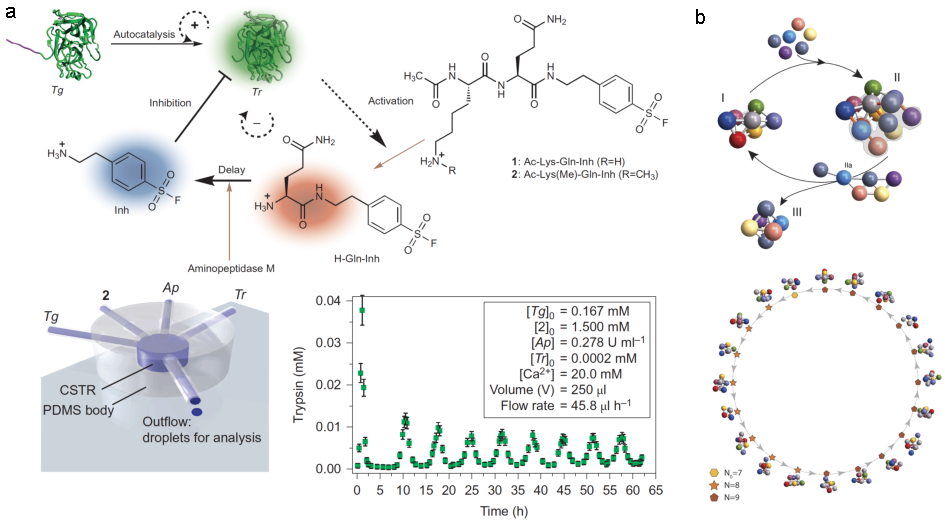
\includegraphics[width=8.5cm]{figures/A5_KeepingTime2.pdf}
    \caption{(a) Chemical reaction network for an enzymatic oscillator.  The enzyme Trypsin (Tr) catalyzes its own production from the inactive form Trypsinogen (Tg) and also the activation of its own inhibitor (Inh). Importantly, the production of the inhibitor is delayed in time, resulting in concentration oscillations of Trypsin within a continuously stirred tank reactor (CSTR). \kbnote{(Adapted from Ref.~\cite{semenov2015rational} with permission.)} (b) A seven particle cluster (I) catalyzes the formation of an octahedral cluster (III) via specific time-varying interactions (left). Such templating reactions lead to the emergence of  exponentially growing catalytic cycles within a pool of monomers (right). \kbnote{(Adapted from Ref.~\cite{Zeravcic2017} with permission.)}}
    \label{fig:KeepingTime2}
\end{figure}
%%%%%%%%%%%%%%%%%%%%%%%%%%

These and other synthetic oscillators are typically macroscopic---even femtoliter droplets of the BZ reagent contain more than 10 million copies of the oscillating redox complex \cite{Toiya2010, Tompkins2014}. Consequently, questions of oscillator precision are rarely a concern. However, as the number of oscillators decreases, the effects of thermal noise and phase diffusion are expected to grow. Can the BZ reaction or other synthetic oscillators operate coherently on the scale of nanometers \cite{Epstein2016}?  To address these and other questions of fluctuating oscillators, model systems based on colloidal particles may prove useful. Experimental studies have shown that transformations between colloidal assemblies can mimic those found in chemical reactions \cite{Meng2010, Chen2011}. By modulating their interactions in time, theoretical studies have demonstrated the emergence of catalytic cycles among small clusters of colloidal spheres (Fig.~\ref{fig:KeepingTime2}b) \cite{Zeravcic2017, zeravcic2017colloquium}. We note, however, that the precision of cyclic processes powered by time-periodic drives are not bound by the uncertainty relation \cite{Barato2016}. Colloidal systems powered by constant thermodynamic forces, such as collections of electromechanical oscillators \cite{Dou2018}, may therefore be useful in investigating the costs of precision and synchronization in small machines.

%%%%%%%%%%%%%%%%%%%%%%%%%%
\subsection{Powering Motion}

Many living organisms are capable of performing mechanical work to drive motion and transport on scales spanning the molecular to the macroscopic. In natural muscle \cite{Alberts2015}, macroscopic actuation is achieved by hierarchical assemblies of many micron-scale actuators (sarcomeres), in which myosin motors ratchet their way along actin fibers through a series of chemically powered conformation changes and binding events. Acting in concert, these molecular motors give rise to macroscopic stresses of ${\sim}0.1$ MPa, strains of ${\sim}30$\%, and strain rates of up to 500\% s$^{-1}$.  Such performance is not achieved at 100\% efficiency as permitted at constant temperature by classical thermodynamics.  Kinetic models of small machines reveal the fundamental trade-offs between efficiency, power, and fluctuations that constrain motor performance \cite{Pietzonka2016}. Here, we use the driven oscillations of our electromechanical oscillator (Fig.~\ref{fig:KeepingTime}) to perform mechanical work and discuss how motor performance is bound by the uncertainty relation (\ref{eq:TUR}).  We highlight recent efforts in synthesizing molecules and colloids that convert chemical energy into motion and discuss the outstanding challenges of emulating natural muscle.

%%%%%%%%%%%%%%%%%%%%%%%%%%
\subsubsection{An Electromechanical Ratchet}

The electromechanical oscillator described above can be harnessed to produce directed motion or perform mechanical work against an applied load. Figure \ref{fig:PoweringMotion}a shows one strategy for rectifying particle oscillations within channels flanked by an array of asymmetric barriers with period $d$. This approach has been demonstrated experimentally within microfluidic channels \cite{drews2013ratcheted}; however, the concept is also applicable at smaller scales where thermal motions become significant \cite{kowalik2016ratcheted}. The stochastic motion of the particle through the ratcheted channel can be modeled by the periodic Markov network illustrated in Figure \ref{fig:PoweringMotion}b. In the absence of an external load ($f=0$), the affinity $\mathcal{A}$ due to the applied voltage drives the particle through the following sequence of states. First, a positively charged particle transfers charge to the negatively biased electrode ($1\rightarrow2$). Now negatively charged, the particle moves in the applied field to the opposite electrode ($2\rightarrow3$). During this transition, the barrier forces the particle to move either to the right with rate $k_m$ or to the left with rate $\gamma k_m$. The geometric asymmetry of the barrier is designed to favor motion to the right such that $\gamma \ll 1$. After charge transfer at the opposite electrode ($3\rightarrow 4$), the particle again moves preferentially to the right into state 1 of the neighboring unit cell ($4\rightarrow 1^+$). Overall, the particle moves a distance $d$ during each cycle as directed by the asymmetric barriers.

%%%%%%%%%%%%%%%%%%%%%%%%%%
\begin{figure}[ht]
    \centering
    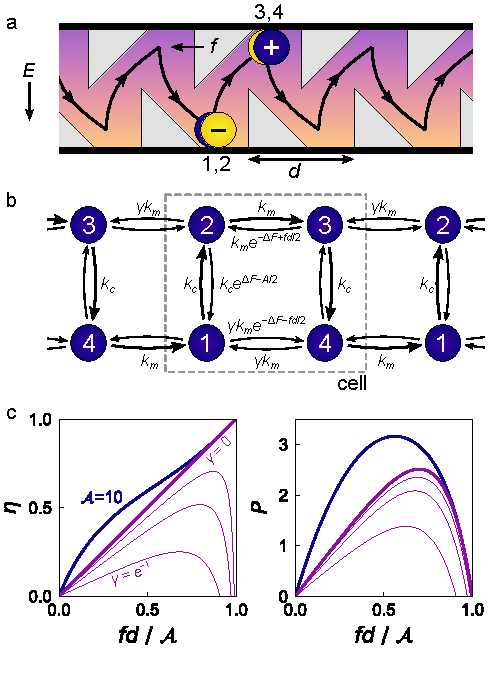
\includegraphics{figures/A5_PoweringMotion.pdf}
    \caption{\textbf{Powering Motion.} (a) Schematic illustration of an electromechanical ratchet based on the oscillator in Figure \ref{fig:KeepingTime}. (b) Markov network for the ratchet showing the transition rates within and between the unit cells. (c) Motor efficiency (left) and power (right) as a function of the applied load for an affinity of $\mathcal{A}=10$. The blue curve denotes the bound (\ref{eq:efficiency}); the purple curves shows the motor performance for $\gamma=e^{-1}, e^{-2}, e^{-3},  \text{ and } 0$.}
    \label{fig:PoweringMotion}
\end{figure}
%%%%%%%%%%%%%%%

Each of the forward transitions is accompanied by a reverse transition whose rate is determined by the detailed balance condition accounting for the free energy difference between the states $\Delta F$, the driving affinity $\mathcal{A}$, and the applied load $f$.  The fluctuating position of the particle $X(t)$ increases or decreases by an amount $d$ upon transition from one unit cell to the next. At steady-state, the average velocity, $v$, of the particle is given by 
\begin{equation}
    v = \frac{\langle X(t)\rangle}{t}= \sum_{ij} p_i (w_{ij}^+ - w_{ij}^-)d
\end{equation}
where $w_{ij}^{\pm}$ denotes the transition rate from state $i$ in the current cell to state $j$ in the cell to the right/left (e.g., $w_{41}^+=k_m$ and $w_{23}^-=\gamma k_m$). Particle motion against the applied load $f$ results in a fluctuating power output $P(t)$ with an average value of $P=fv$. At the same time, this electromechanical motor dissipates energy at an average rate $\sigma$, as specified by the principles of stochastic thermodynamics \cite{Pietzonka2016}.  With these quantities, the thermodynamic efficiency of the motor is given by the fraction of energy supplied to the system that is converted into useful work, $\eta = P / (P+\sigma)$. In addition to the average power and efficiency, the motor is further distinguished by its constancy, as characterized by power fluctuations
\begin{equation}
    \Delta_P = \lim_{t\rightarrow \infty}\langle (P(t)-P)^2 \rangle t = 2 D f^2
\end{equation}
where $D$ is the dispersion of the particle position.

These three quantities---the power $P$, efficiency $\eta$, and constancy $\Delta_P$---are constrained by the thermodynamic uncertainty relation \cite{Pietzonka2016} as 
\begin{equation}
    \eta \leq \frac{1}{1+2P/\Delta_p} \label{eq:efficiency}
\end{equation}
This universal result suggests two fundamentally different strategies for improving the efficiency of a stochastic motor.  First, one can operate near equilibrium such that the average power vanishes ($P\rightarrow0$) with finite power fluctuations (Fig.~\ref{fig:PoweringMotion}c).  Like a clock without precision, a motor without power is of little practical value regardless of its efficiency.   An alternate route to achieving maximum efficiency is increasing the power fluctuations ($\Delta_p\rightarrow\infty$) at finite power; however, large fluctuations may be unacceptable for certain applications.  In the face of competing performance criteria, the ``optimal'' motor depends on the context.

Like related models of molecular machines \cite{Pietzonka2016}, the electromechanical ratchet has a maximum efficiency of $\eta=f d/\mathcal{A}$ in the limit of perfect biasing ($\gamma\rightarrow 0$).  In this limit, the energy $\mathcal{A}$ supplied during each step contributes a fixed amount $f d$ to the total work performed.  For a driving affinity $\mathcal{A}=10$, the efficiency at maximum power is 70\% assuming fast charging ($k_c/k_m\rightarrow\infty$); the fundamental bound under these conditions is 73\% (Fig.~\ref{fig:PoweringMotion}c).  While detrimental to motor efficiency, the uneven allocation of dissipation among the different steps is often beneficial in increasing power output \cite{brown2017allocating}. 

%%%%%%%%%%%%%%%%%%%%%%%%%%
\subsubsection{From Molecular Motors to Artificial Muscles}

Nature's molecular machines perform mechanical work driven by constant thermodynamic forces such as the chemical potential difference between ATP and ADP in their surroundings.  By contrast, most synthetic molecular motors require step-wise changes in their environment to drive the completion of thermodynamic cycles necessary to perform directed motion or mechanical work \cite{coskun2012great, Erbas-Cakmak2015, kassem2017artificial, pezzato2017mastering}.  Notable exceptions include the light-driven molecular rotors pioneered by the Feringa group, which rotate continuously upon light irradiation \cite{koumura1999light}.  These small machines are no small achievement as evidenced by the 2016 Nobel prize in chemistry to Sauvage \cite{sauvage2017chemical}, Stoddart \cite{Stoddart2017} and Feringa \cite{Feringa2017}. In the same year, Leigh and coworkers demonstrated the first ever molecular machine driven by a steady chemical gradient  (Fig.~\ref{fig:PoweringMotion2}a) \cite{Wilson2016}. A small molecular ring performs a biased random walk around a cyclic asymmetric track propelled by the (nearly) irreversible consumption of chemical fuel. Beyond these landmark achievements, outstanding challenges remain in integrating such molecular machines into macroscopic materials and in coupling their activity to other chemical processes.  For example, the recent demonstration of a molecular motor driven by pH oscillations \cite{Erbas-Cakmak2017} suggests opportunities for integrating motion with time keeping via pH-regulated chemical oscillators \cite{orbán2015ph}.

%%%%%%%%%%%%%%%%%%%%%%%%%%
\begin{figure}[h!]
    \centering
    \includegraphics[width=8.5cm]{figures/A5_PoweringMotion2.pdf}
    \caption{(a) Operation of a chemically fuelled catenane rotary motor. The benzylic amide macrocycle (blue) binds to one or other of the two fumaramide sites (green) of the cyclic track. Bulky groups (red) sterically block passage of the small blue ring and trap it in one compartment or the other. Cleavage of one of the bulky groups through a chemical reaction (loss of orange sphere) allows the small ring to shuttle back and forth between the two fumaramide sites on the track via Brownian motion along the unblocked pathway. If the kinetics for blocking group attachment are faster when the small ring is far from the reactive site, but the cleavage reaction occurs at a rate independent of the small ring position, then the small ring will directionally rotate around the larger one. \kbnote{(Adapted from Ref.~\cite{Wilson2016} with permission.)} (b) Left: The  hybrid contains covalent chains grafted radially from the nanofiber surface. Right and bottom: Circumferentially aligned hybrid polymer shows anisotropic contraction along the length of the tube upon heating. \kbnote{(Adapted from Ref.~\cite{chen2018artificial} with permission.)} (c) Self-electrophoresis mechanism of platinum-gold nanorods. The asymmetric reactions on the rod lead to an asymmetric charge density distribution, which results in fluid motion from the platinum to the gold end and motion of the (negatively charged) particle with the platinum end forward. \kbnote{(Adapted from Ref.~\cite{Moran2017} with permission)}}
    \label{fig:PoweringMotion2}
\end{figure}
%%%%%%%%%%%%%%%%%%%%%%%%%%

As in biology, the realization of one function is often intertwined with another. Creating active soft matter with the capabilities of natural muscle requires integrating molecular actuation and assembly to create anisotropic, hierarchically ordered materials.  Inspired by muscle, Stupp and co-workers developed an anisotropic hydrogel actuator comprised of long supramolecular fibers decorated with thermoresponsive polymers \cite{chin2018covalent}.  Long ranged order among the fibers allowed for large anisotropic strains upon changes in temperature.  As in other hydrogel actuators the rate of actuation was limited by transport of water into or out of the gel. More generally, the realization of active soft matter on macroscopic scales requires careful consideration of the transport processes necessary to maintain open thermodynamic systems. A related advance from Feringa and co-workers achieves material actuation using light-driven motors coupled to supramolecular fibers, thereby eliminating the need for mass transfer (Fig.~\ref{fig:PoweringMotion2}b) \cite{chen2018artificial}.

At the microscale, active colloids based on self-phoretic propulsion convert chemical energy into motion and work by an entirely different mechanism (Fig.~\ref{fig:PoweringMotion2}c) \citep{illien2017fuelled, Moran2017}. The asymmetric production or consumption of chemical species at the surface of a colloidal particle creates interfacial forces that drive self-diffusiophoretic or self-electrophoretic fluid flows that propel particle motion.  The motions of individual particles can be rationally engineered by tailoring particle shape and surface chemistry \cite{Brooks2018shape}.  Together, ensembles of chemically powered active colloids interact via non-reciprocal forces to drive the formation of dynamic assemblies (see below) \cite{wang2015one, Lowen2018}.  A significant limitation of these systems, however, is their poor efficiency: only a small fraction of the chemical energy consumed (ca.~$10^{-9}$) is dissipated via mechanical motion \cite{wang2013understanding}. It is therefore desirable to improve the performance of current mechanisms based on self-phoresis or to identify other approaches for chemical-to-mechanical energy transduction at colloidal scales (e.g., bubble propulsion \cite{li2016rocket}). 

%%%%%%%%%%%%%%%%%%%%%%%%%%
\subsection{Building structures}

Unlike the dynamic functions of keeping time and powering motion, external energy input is not required to build and maintain material structures.  Within the living cell, there exist many structures that appear to be equilibrium assemblies: lipid membranes, protein complexes, and membrane-less organelles among others.  We now know, however, that many of these ``structures'' are actually built and maintained by dissipative processes.  The assembly of tubulin dimers into microtubles and their catastrophic disassembly (so-called dynamic instability) provide a canonical example \cite{Desai1997}. As evolution is rarely wasteful, dissipative assembly processes must provide these materials and the organism with dynamic functions that justify the thermodynamic costs \cite{Ragazzon2018}. One benefit of dissipative self-assembly \cite{De2018} is greater temporal control over the assembly and disassembly of material structures.  Here, we describe a simple model that illustrates how energy input can greatly accelerate the rates of assembly and disassembly without qualitatively disrupting the phase behavior of equilibrium structures \cite{marsland2018active}. 

%%%%%%%%%%%%%%%%%%%%%%%%%%
\subsubsection{A Dissipative Nanoparticle Assembly}

To illustrate the costs and benefits of active assembly processes, we consider the formation of a tetrahedral cluster of nanoparticles interacting via light-activated solvophobic interactions (Fig.~\ref{fig:BuildingStructures}a). This example is inspired by the light-induced assembly of gold nanoparticles functionalized with azobenzene ligands \cite{klajn2007light}.  Each nanoparticle is assumed to exist in two possible states denoted ``active'' and ``inactive'', corresponding to particle surfaces enriched in the cis and trans azobenzene isomers, respectively.  The free energy of the active state is higher than that of the inactive state by a factor $\Delta F$; energy input is therefore required to drive particles into the active state.  Specifically, the rate of energy dissipation required to maintain a concentration ratio $\rho=c_A/c_I> e^{-\Delta F}$ is bounded by 
\begin{equation}
    \sigma \geq \left[\frac{ k_I (\rho - e^{-\Delta F})}{1+\rho}\right] (\ln\rho+\Delta F),
\end{equation}
where $k_I$ is the transition rate for the undriven process. The equality holds only when the rate of the driven transition is fast such that $k_A/k_I\rightarrow \infty$ \cite{Horowitz2017}. This general bound on the dissipation rate has been proven to apply for arbitrary Markov networks \cite{Horowitz2017}.

%%%%%%%%%%%%%%%%%%%%%%%%%%
\begin{figure}[h!]
    \centering
    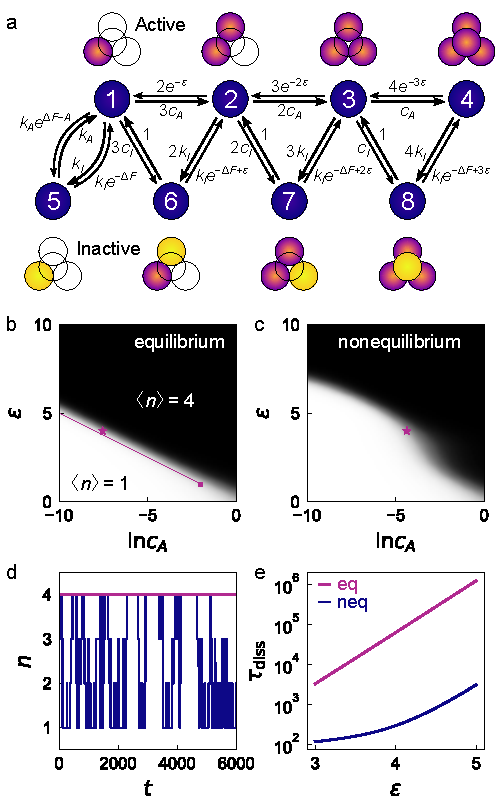
\includegraphics{figures/A5_BuildingStructures.pdf}
    \caption{\textbf{Building Structures.} (a) Markov network for the dissipative self-assembly of a tetrahedral cluster. The purple, yellow, and open circles represent ``active'' particles, ``inactive'' particles, and unoccupied sites, respectively. (b) Equilibrium phase diagram based on states 1 to 4. The grayscale map denotes the average occupancy of the cluster, $\langle n\rangle$. The solid line and the square marker denote the phase boundary and the critical point, respectively, in the thermodynamic limit of large clusters. (c) Nonequilibrium phase diagram for parameters $\Delta F=6$, $\ln c_I = -6$, and $k_I = 0.01$.  (d) Fluctuating occupancy $n$ for the equilibrium (purple) and nonequilibrium (blue) systems for an interaction strength $\varepsilon=4$ at phase coexistence (star markers in a and b). (e) Mean first passage time $\tau_{\text{diss}}$ from the assembled to the disassembled state ($4\rightarrow1$) for the equilibrium (purple) and nonequilibrium (blue) systems as a function of the interaction strength $\varepsilon$. }
    \label{fig:BuildingStructures}
\end{figure}
%%%%%%%%%%%%%%%%%%%%%%%%%%

Given that it costs a steady supply of energy to maintain disequilibrium in the active particle concentration, what is the benefit? In short, the answer is speed in assembling and/or disassembling particle structures. To show this, consider that the active particles interact with one another through attractive, short ranged interactions with a free energy gain $\varepsilon$ for each pairwise bond formed. We will assume that inactive particles do not interact with each other or the active particles. As summarized by the Markov network in Figure \ref{fig:BuildingStructures}a, active particles are added to the growing cluster with a diffusion-limited rate $k_{\text{on}} c_A$.  Active particles within the cluster become inactive with a rate $k_I$ and detach from the cluster at a rate $k_{\text{off}}$.  We set $k_{\text{on}}$ and $k_{\text{off}}$ equal to unity, such that time is measured in units of $k^{-1}_{\text{off}}$ and concentration in units of $k_{\text{off}}/k_{\text{on}}$.

Figures \ref{fig:BuildingStructures}b and \ref{fig:BuildingStructures}c compare the equilibrium phase behavior to that of the active system.  For the equilibrium assemblies, we consider only states 1 to 4 and plot the average number of particles within the cluster $\langle n\rangle$ as a function of the monomer concentration $c_A$ and the interaction energy $\varepsilon$.  For strong interactions or high monomer concentrations, the clusters are fully occupied $\langle n\rangle\rightarrow 4$ (Fig.~\ref{fig:BuildingStructures}b, black region).  For weak interactions or low monomer concentrations, the particles do not assemble $\langle n\rangle \rightarrow 1$ (Fig.~\ref{fig:BuildingStructures}b, white region).  Below the critical point (Fig.~\ref{fig:BuildingStructures}b, purple circle), coexistence of the assembled and disassembled states is reasonably well approximated by the thermodynamic result, $\varepsilon = -2\ln c_A$, which describes the limit of large clusters $N\rightarrow\infty$ \cite{marsland2018active}.  Driving the system away from equilibrium acts to perturb the coexistence boundary; however, the qualitative features of the phase diagram are similar to those at equilibrium (Fig.~\ref{fig:BuildingStructures}c). 

The dynamics of the two systems, however, are dramatically different.  For coexistence at equilibrium (i.e., when $p_1=p_4$), the characteristic time required to disassemble the tetrahedral cluster scales as $\tau_{\text{diss}}\sim e^{3\varepsilon}$.  The rate limiting step is the removal of one particle from the cluster ($4\rightarrow 3$), which results in the loss of three interparticle bonds.  For strong interactions ($\varepsilon\gg1$), the time scales required for assembly and disassembly become quite large.  By contrast, the dissipative structure has an alternate route for disassembly ($4\rightarrow 8\rightarrow 3$), which can be orders of magnitude faster than that of the equilibrium structure.  Figure \ref{fig:BuildingStructures}d shows the fluctuating occupancy of the cluster at coexistence for both the equilibrium and active systems with a common interaction energy of $\varepsilon=4$.  During this time period, the equilibrium system remains in the assembled state while the active system assembles and disassembles repeatedly.  The characteristic time for disassembly---defined as the mean passage time from state 4 to 1---is more than two orders of magnitude smaller for the active system than the equilibrium system (Fig.~\ref{fig:BuildingStructures}e). 

%%%%%%%%%%%%%%%%%%%%%%%%%%
\subsubsection{Dissipative Self-Assembly of Synthetic Materials}

Inspired by the cell cytoskeleton, the dissipative self-assembly of supramolecular materials has emerged as a promising strategy for controlling material organization in time as well as space \cite{VanRossum2017, De2018}. In contrast to equilibrium assemblies, where the rates of assembly and disassembly are related by detailed balance, dissipative self-assembly uses two or more processes to independently control the rates at which structures grow and degrade.  This basic concept has been applied to create a growing variety of supramolecular polymers \cite{Sorrenti2017} that exhibit simultaneous growth and shrinkage \cite{boekhoven2015transient}, tunable lifetimes \cite{Tena-Solsona2017}, conformational switching \cite{dhiman2017transient}, and nonequilibrium fluctuations \cite{boekhoven2015transient} reminiscent of dynamic instability in microtubules. In one pioneering study, small molecule building blocks were activated for assembly by reaction with a chemical fuel and subsequently degraded to their original inactive form by a different reaction pathway (Fig.~\ref{fig:BuldingStructure2}a) \cite{boekhoven2015transient}. As in the model above, the breaking of detailed balance enabled the formation of supramolecular assemblies that exhibit ``low-temperature'' phase behavior with ``high-temperature'' kinetics \cite{marsland2018active}.  Active soft matter with tunable lifetimes may be useful as self-erasing inks or as self-destructing hydrogels for tissue regeneration or drug release \cite{Rieß2018}.

%%%%%%%%%%%%%%%%%%%%%%%%%%
\begin{figure}[h!]
    \centering
    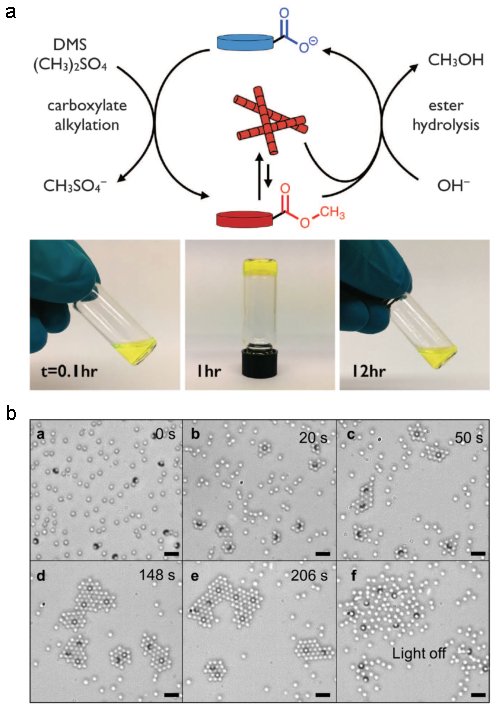
\includegraphics[width=8.5cm]{figures/A5_BuildingStructures2.pdf}
    \caption{(a) The dissipative  self-assembly of supramolecular materials forming the transient structure. Up: In a typical reaction cycle, carboxylate groups on the inactive self-assembling building blocks  react with the fuel, DMS, to produce methyl esters. These activated building blocks self-assemble into fibrous structures. Methyl esters can hydrolyze both in the assembled and free states to revert to the original inactive building block. One full cycle produces $CH_3OH$ (methanol) and $CH_3SO_4$(MMS) as waste products. Bottom: A typical sample in a reaction cycle at t = 0.1, 1, and 12 hours, with 1 mM of fluorescein added for coloring. \kbnote{(Adapted from Ref.~\cite{boekhoven2015transient} with permission.)}  (b) Photo-switchable assembly of a colloidal structure. A sequence of images showing the growth of crystals under full UV illumination. Active particles can be distinguished from the passive ones by the dark crescent or ring at their edge. Crystals melt by thermal diffusion when the light is turned off. \kbnote{(Adapted from Ref.~\cite{Singh2017} with permission.)} }
    \label{fig:BuldingStructure2}
\end{figure}
%%%%%%%%%%%%%%%%%%%%%%%%%%

In addition to molecular building blocks, the formation of dissipative structures by breaking detailed balance can also be applied to photoswitchable nanoparticles \cite{klajn2007light, kundu2015light, manna2015orthogonal, he2016light} and active colloids \cite{Soto2014, soto2015self, Niu2017, Singh2017, Schmidt2018} (Fig.~\ref{fig:BuldingStructure2}b). A particularly illustrative example is provided by a class of colloidal assemblies dubbed active colloidal molecules \cite{Lowen2018}, in which colloidal particles move due to concentration gradients created by themselves and their neighbors \cite{Soto2014}.  These dissipative structures appear to violate action-reaction symmetry---for example, two otherwise stationary particles may come together to form a stable, self-propelled cluster \cite{Soto2014}.  These and other motions are sustained by the steady supply or removal of chemical species at the particle surface (e.g., due to a catalytic reaction \cite{Singh2017} or release from the particle interior \cite{Niu2017}).  Interestingly, these dissipative assemblies are predicted to exhibit time-dependent functionality such as oscillatory deformations and run-and-tumble propulsion \cite{soto2015self}.  More generally, this example highlights the importance of feedback between structures and processes necessary for creating dynamic functions (Fig.~\ref{fig:1}b). Colloidal particles move in response to chemical gradients they create, and the gradients in turn are shaped by the particle configuration.  Beyond colloids, this basic strategy was recently employed to create acoustic metamaterials with dynamically tunable bandgaps \cite{bachelard2017emergence, bishop2017acoustic}; other realizations of dissipative self-assembly are sure to follow. 

%%%%%%%%%%%%%%%%%%%%%%%%%%
\subsection{Making Copies}

The dynamic functions of living matter trace their origins to the single function of ``making copies'', which provides the basis for evolution by natural selection.  Replication of the genetic code by molecular machines---namely, DNA polymerase---occurs with incredible fidelity characterized by an error rate of as small as $10^{-9}$ \cite{McCulloch2008}. This level of precision is critical in avoiding deleterious mutations, which can lead to improper function and even death of the organism. It has long been recognized that making such accurate copies requires energy dissipation \cite{Bennett1979}; however, the details of the dissipation-error trade-off depend on the specific proofreading mechanism \cite{Sartori2013}. DNA replication is but one important part of cellular reproduction, whereby the living cell creates a copy of itself---including both its internal structures and processes.  Here, we consider the comparably simple problem of creating a self-replicating material structure that contains some minimal amount of combinatorial information. We present a model for the self-replication of DNA origami rafts inspired by the experiments of Seeman and Chaikin \cite{He2017} (Fig.~\ref{fig:MakingCopies}) and discuss other routes toward the realization of self-replicating, evolvable matter.

%%%%%%%%%%%%%%%%%%%%%%%%%%
\subsubsection{A minimal replicator}

In the model, two monomers $A$ and $T$ can combine to form four possible dimers $AA$, $AT$, $TA$, and $TT$, each of which catalyzes its own formation.  We focus our attention on a particular dimer $AT$ and its function as a catalyst for the production of itself and the other `mutant' dimers (Fig.~\ref{fig:MakingCopies}a). During a successful replication cycle, the monomers $A$ and $T$ present in solution first bind to the seeded $AT$ template through complementary interactions.  Once bound, the monomers react to form a new $AT$ dimer that dissociates from the template to complete the cycle.  In addition to this ``correct'' cycle, we consider one of the ``incorrect'' cycles that leads to formation of the mutant $TT$; other types of errors are excluded to simplify the analysis.  The resulting model is described by a 6-state Markov network containing two cycles with currents $J_c$ and $J_i$ that quantify the production of the correct and incorrect dimers, respectively (Fig.~\ref{fig:MakingCopies}b).  In assessing replicator performance, we examine how the rate of copying $J_c$ and the error fraction $\eta = J_i/J_c$  depend on the dissipation rate. 

%%%%%%%%%%%%%%%%%%%%%%%%%%
\begin{figure}[h!]
    \centering
    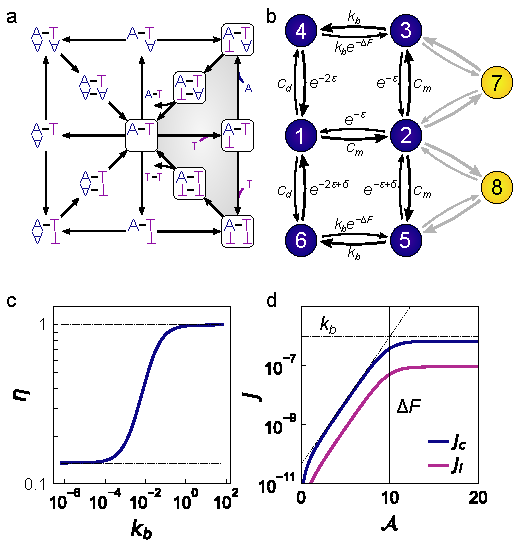
\includegraphics{figures/A5_MakingCopies.pdf}
    \caption{\textbf{Making Copies.}(a) Reaction network showing dimer formation catalyzed by the $AT$ template. (b) Markov network and transition rates corresponding to the shaded region of the network in (a). The additional states 7 and 8 correspond to a simple kinetic proofreading scheme. (c) Error fraction $\eta$ as a function of the bonding rate $k_b$ for $\Delta F = 10$, $\varepsilon = 6$, and $\delta=2$. For $k_b\ll e^{-\varepsilon+\delta/2}$, the error rate approaches its minimal value of $\eta=e^{-\delta}$. (d) Rate of formation for correct and incorrect dimers, $J_c$ and $J_i$, as a function of the driving affinity $\mathcal{A}$ for $c_m=e^{-4}$; other parameters are listed in (c). }
    \label{fig:MakingCopies}
\end{figure}
%%%%%%%%%%%%%%%%%%%%%%%%%%

In the model, monomers and dimers bind to the template with diffusion limited rates proportional to their respective concentrations in solution, $c_m$ and $c_d$ (Fig.~\ref{fig:MakingCopies}b). The rates of dissociation depend on the interaction energies, denoted $\varepsilon$ for $AT$ and $\varepsilon-\delta$ for $TT$. These monomer interactions combine in an additive fashion to determine the binding energy between two dimers. Bond formation between the bound monomers occurs at a rate $k_b$ with a free energy of reaction $\Delta F$.  Assuming equal concentrations of $AT$ and $TT$ dimers in solution, the driving affinity is $\mathcal{A} = 2\ln(c_m/c_d) + \Delta F$ for both the correct and incorrect replication cycles.  We assume that the bond energy is sufficiently large to inhibit spontaneous degradation of the dimers, $\Delta F\gg1$; the monomer binding energies are smaller by comparison such that $\Delta F> \varepsilon>\delta >0 $.

To minimize replication errors, the rate of bond formation should be sufficiently slow such that monomers equilibrate onto the catalyst template $AT$---that is, $k_b\ll e^{-\varepsilon + \delta/2}$ (Fig.~\ref{fig:MakingCopies}c). Under these conditions, the error fraction approaches $\eta = e^{-\delta}$ where $\delta$ is the difference in the binding energies of the correct and incorrect monomers.  If we operate in this high accuracy regime, a finite driving affinity is required to drive replication at a rapid rate (Fig.~\ref{fig:MakingCopies}d).  Optimal performance requires that monomers bind ($c_m>e^{-\varepsilon}$) while dimers unbind ($c_d<e^{-2\varepsilon}$), which implies large affinities, $\mathcal{A}>\Delta F$.  The model suggests that fast and accurate replication proceeds at a rate $J_c\sim k_b\ll e^{-\varepsilon+\delta/2}$ and dissipates at least $\Delta F$ per cycle. 

Additional energy input can allow for further improvements to replication accuracy through various forms of kinetic proofreading \cite{Hopfield1974, Murugan2012}.  In its simplest form, we consider two additional states---denoted 7 and 8---in which the $AT:T$ complex binds to modified monomers $A^*$ and $T^*$, respectively (Fig.~\ref{fig:MakingCopies}b). Once bound, the modified monomers convert to their native forms $A$ and $T$ prior to bond formation.  Steady currents around the proofreading cycles ($2\rightarrow7\rightarrow3$ and $2\rightarrow8\rightarrow5$) are powered by cycle affinities $\mathcal{A}_p$ due to the chemical potential difference between the modified and unmodified monomers in the surrounding reservoir.  By engineering the transition rates along these auxiliary cycles, the error fraction can be reduced to a minimum value of $\eta\rightarrow e^{-2\delta}$ \cite{Hartich2015}. Further improvements can be achieved using increasingly sophisticated proofreading networks \cite{Murugan2012}.

%%%%%%%%%%%%%%%%%%%%%%%%%%
\subsubsection{Self-replicating materials}

The pursuit of material structures capable of self-replication is motivated by the promise of revolutionary advances in materials synthesis and design \cite{He2017}. Given sufficient resources, the number of self-replicating structures grows exponentially with time thereby accelerating rates of material synthesis.  Perhaps more importantly, the ability to direct the evolution of replicating materials through application of selective pressures could facilitate the design of complex structures with desired functions.  At the molecular scale, the study of self-replication has long sought to provide useful insights into the chemical origins of life itself \cite{Orgel1992,ruiz2013prebiotic}. In this context, it is useful to distinguish self-replication of combinatorial information from simpler forms of autocatalysis that copy a single structure (not one of many possible structures) \cite{schulman2012robust}. Several mechanisms for autocatalysis have been explored including template-based copying \cite{Wang2011, He2017},  crystal growth and fragmentation \cite{Viedma2005,carnall2010mechanosensitive}, and catalytic reaction networks (hypercycles) \cite{Eigen1977, Zeravcic2014}. Combined with combinatorial information such as heterogeneous polymer sequences or macromolecular assemblies (Fig.~\ref{fig:MakingCopies2}a) \cite{sadownik2016diversification}, any form of autocatalysis with sufficient fidelity \cite{Eigen1988} can enable the creation of self-replicating materials.

Materials based on DNA \cite{Jones2015} possess several attributes useful in the development of self-replicating structures \cite{Wang2011, schulman2012robust, He2017}.  First, large amounts of combinatorial information can be encoded within sequences of nucleotide bases. Second, the specific interactions between complementary base pairs enables the programmable folding and assembly of complex structures.  These specific interactions of tunable strength can also be used to achieve autocatalysis via template-based copying \cite{Wang2011, He2017}.  In a recent work, Seeman and Chaikin showed how the replication of DNA origami rafts can lead to exponential growth with more than 7,000,000-fold amplification of the original seeded structure \cite{He2017}.  Strong, specific monomer-template interactions resulted in high fidelity copies but required cyclic energy inputs to promote monomer binding (low temperature), bond formation (UV light), and dimer unbinding (high temperature) (Fig.~\ref{fig:MakingCopies2}b). While thermodynamically costly, such external cycles offer significant practical benefits in controlling the replication process.  Remarkably, the seeding of two competing structures led to exponential growth and selection of the ``fittest'' structure, as determined by the replicator environment (namely, the pH).

%%%%%%%%%%%%%%%%%%%%%%%%%%%%%%%%%
\begin{figure}[h]
    \centering
    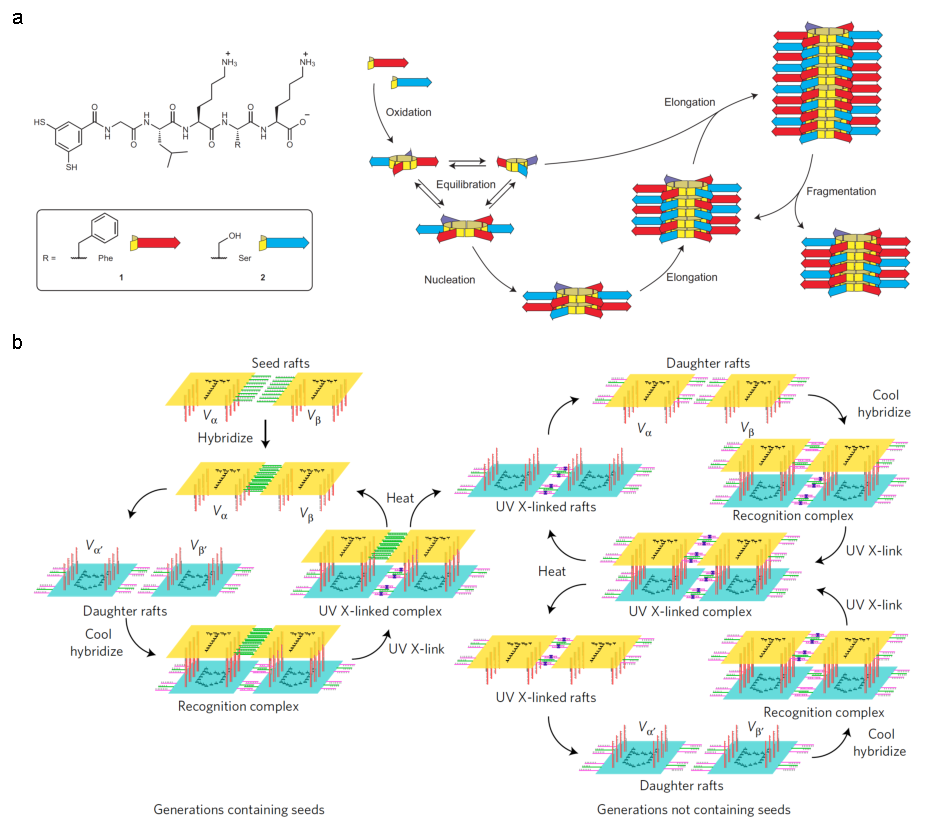
\includegraphics[width=8.5cm]{figures/A5_MakingCopies2.pdf}
    \caption{(a) Left: Structures of building blocks. Right: Mechanism of replication in a two-component system: the building blocks form an exchanging mixture of macrocycles of different sizes and building-block compositions via oxidation of thiols to give disulfide bonds and subsequent disulfide exchange. The hexamer macrocycles self-assemble into fibres as the peptide chains (arrows) form $\beta$-sheets through a nucleation–elongation mechanism. The fibres grow from their ends and break on mechanical agitation, which doubles the number of fibre ends that further promote the formation of self-replicating hexamer. \kbnote{(Adapted from Ref.~\cite{sadownik2016diversification} with permission.)} (c) Self-replication cycling of the dimer seed system, including ‘TT’ seed formation with special horizontal complementary sticky ends, recognition and hybridization of daughter rafts to seeds with two sets of vertical bonds ($V\alpha$ to $V\alpha^{'}$ , $V\beta$ to $V\beta^{'}$), formation of new-generation dimers using horizontal bonds and the $^{CNV} K$ photocrosslinking reaction and separation of the two successive generations by heating the system. The cycles on the left include seed rafts and those on the right do not. \kbnote{(Adapted from Ref.~\cite{He2017} with permission.)}  }
    \label{fig:MakingCopies2}
\end{figure}
%%%%%%%%%%%%%%%%%%%%%%%%%%%%%%%%%

Beyond DNA nanostructures, assemblies of micro- and nanoscale colloids interacting via DNA-based linkers \cite{leunissen2009towards}, magnetic dipoles \cite{zhang2014self, dempster2015self}, or toggled interactions \cite{zhang2014accelerated,sherman2016dynamic} are also promising candidates for self-replicating materials. The replication of 3D colloidal assemblies presents significant challenges for template-based copying strategies due to the presence of internal structural features that are inaccessible to components of the daughter structure.  One way around this challenge is to separate replication and assembly using flexible 1D assemblies, which unfold prior to replication and then reassemble into 3D structures \cite{cademartiri2014programmable}.  Alternatively, 3D clusters can be replicated with in larger catalytic networks in which structural features on one cluster template the formation of a second cluster and vice versa \cite{Zeravcic2014}.  Such catalytic cycles are predicted to emerge spontaneously within mixtures of colloidal spheres with specific time-varying interactions \cite{Zeravcic2017}.

%%%%%%%%%%%%%%%%%%%%%%%%%%
%%%%%%%%%%%%%%%%%%%%%%%%%%
\section{Conclusions}

The four dynamic functions considered here---keeping time, powering motion, building structures, and making copies---only begin to explore the diverse and creative solutions by which living organisms survive and thrive in complex non-equilibrium environments. In particular, we have largely omitted the discussion of functions related to computation and information processing, which remains an active area of statistical physics \cite{Parrondo2015, Lutz2015}. The ability to create material systems that sense their environment \cite{della2018fuel}, communicate with one another \cite{chen2013programmable}, and perform complex computations \cite{fang2016pattern} will benefit from an understanding of the fundamental connections between entropy and information. The creation of active soft matter on macroscopic scales will require careful consideration of transport processes, by which matter and energy are delivered to and removed from the material system. In biology, active transport mechanisms are favored over passive diffusion for length scales exceeding few microns \cite{soh2010reaction}. At larger scales, dissipative materials will likely benefit from the incorporation of synthetic vasculatures or other forms of active transport. The integration of multiple functions within material systems will require new levels of regulatory and control functions \cite{he2012synthetic} analogous to those of the living cell. Such functions are critical to realizing the full potential of soft robotics \cite{whitesides2018soft} to create ``life-like'' machines. It remains uncertain whether or not the capabilities of living matter will ever be matched by synthetic materials engineered to organize spontaneously and function autonomously. There is only one way to find out.
\end{appendices}